\documentclass[class=article,border=5pt,tikz]{standalone}
\usetikzlibrary{matrix}

\tikzset{
  square matrix/.style={
    matrix of nodes,
    column sep=-\pgflinewidth, row sep=-\pgflinewidth,
    nodes={
      rectangle,
      draw=black,
      minimum height=#1,
      anchor=center,
      align=center,
      text width=#1,
      text height=2ex,
      text depth=0.5ex,      
      inner sep=0pt,
    }    
  },
  square matrix/.default=2.5em
}

\newcommand{\x}{\phantom{$-00$}}

\begin{document}
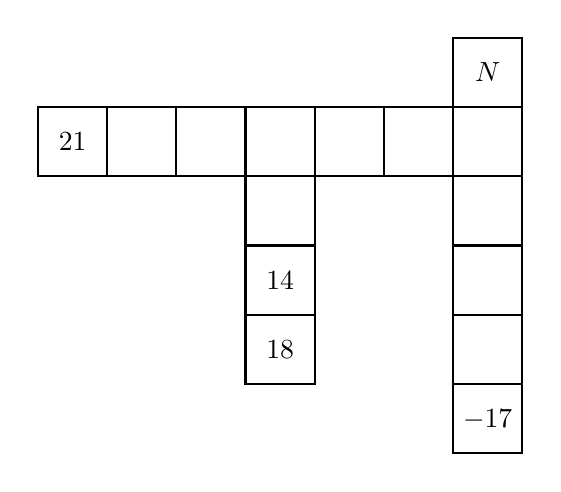
\begin{tikzpicture}[thick]
\matrix[square matrix]
{
       &       &       &       &       &        &  $N$ \\
  $21$ &    \x &    \x &    \x &    \x &     \x &   \x \\
       &       &       &    \x &       &        &   \x \\
       &       &       &    14 &       &        &   \x \\
       &       &       &    18 &       &        &   \x \\
       &       &       &       &       &        & $-17$ \\
};
\end{tikzpicture}

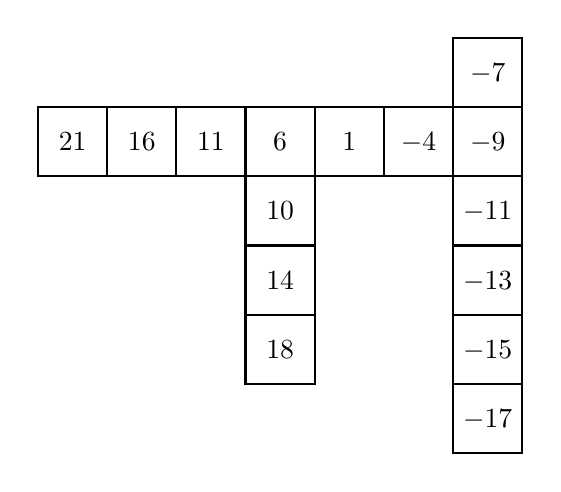
\begin{tikzpicture}[thick]
\matrix[square matrix]
{
       &       &       &       &       &        &  $-7$ \\
  $21$ &  $16$ &  $11$ &   $6$ &   $1$ &   $-4$ &  $-9$ \\
       &       &       &    10 &       &        & $-11$ \\
       &       &       &    14 &       &        & $-13$ \\
       &       &       &    18 &       &        & $-15$ \\
       &       &       &       &       &        & $-17$ \\
};
\end{tikzpicture}
\end{document}